\section{Assiomi dei numeri reali}
\begin{itemize}
    \item Assiomi relativi alle operazioni
    \item Assiomi relativi all'ordinamento
    \item Assioma di completezza
\end{itemize}

\subsection{Assiomi relativi alle operazioni}
Sono definite le operazioni di addizione e moltiplicazione tra coppie di numeri
reali e valgono le proprietà:
\begin{itemize}
    \item \textbf{Proprietà associativa}
    \item \textbf{Proprietà commutativa}
    \item \textbf{Proprietà distributiva}
    \item \textbf{Esistenza degli elementi neutri}
    \item \textbf{Esisstenza degli opposti}
    \item \textbf{Esistenza degli inversi}
\end{itemize}

\subsection{Assiomi relativi all'ordinamento}
E' definita la relazione di Minore o Uguale $\leq$.
\begin{itemize}
    \item \textbf{Dicotomia}
    \item \textbf{Proprietà Assimetrica}
    \item \textbf{Assioma di completezza}
\end{itemize}

\subsubsection{Assioma di completezza}
\[
    \forall a \in A, \forall b \in A, a \leq b  \implies \exists c \in A : a \leq c \leq b
\]
\textbf{Esempi:}\\
\begin{figure}[h]
    \centering
    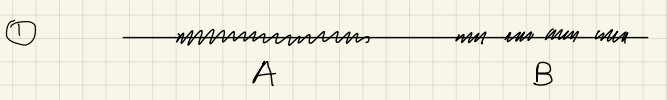
\includegraphics[width=0.3\textwidth]{1.png}
    \caption{Esempio 1}
    \label{fig:1}
\end{figure}

Esistono infiniti c.

\begin{figure}[!ht]
    \centering
    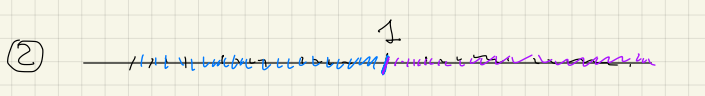
\includegraphics[width=0.3\textwidth]{2.png}
    \caption{Esempio 2}
    \label{fig:2}
\end{figure}
\[
    A = \{x \in \R : x \geq 1\} \ \ \ B = \{x \in \R : x \geq 1\} \implies c = 1
\]
\textbf{Osservazione:} Non tutti gli insiemi hanno il più grande o il più piccolo elemento. Ad esempio:
\[
    A = \{1, \frac{1}{2}, \frac{1}{3}, \frac{1}{4}, \cdots, \frac{1}{n}, \cdots\} = \{\frac{1}{n} : n\in \mathbb{N}\}
\]
\begin{figure}[h]
    \centering
    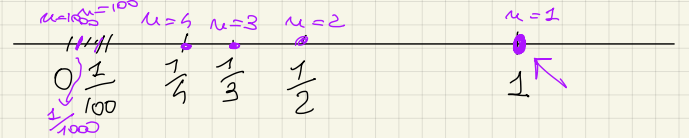
\includegraphics[width=0.3\textwidth]{3.png}
    \caption{Esempio 3}
    \label{fig:3}
\end{figure}

Non ha un elemento più piccolo. (Invece c'è il più grande che è $1$).

\subsection{Denso}
Si dimostra che $\mathbb{Q}$ è denso sulla retta reale (nel senso che fra due
numeri razionali è sempre possibile trovare un terzo, anzi infiniti).

\[
    a = \frac{m_1}{n_1} \ \ \ b = \frac{m_2}{n_2}
\]
faccio la media $\frac{a+b}{2} =\frac{\frac{m_1}{n_1} + \frac{m_2}{n_2}}{2} =
    \frac{m_1n_2 + m_2n_1}{2n_1n_2} \implies \in \mathbb{Q}$

\subsubsection{$\sqrt{2}$}
$\sqrt{2}$ non si può rappresentare come numero razionale.\\
\textbf{Dimostrazione:} Ragioniamo per assurdo, supponiamo che $\sqrt{2}$ sia un numero razionale, cioè $\sqrt{2} = \frac{m}{n}$ con $m,n \in \mathbb{Z}$ posso supporre che $m. n$ siano primi tra loro e che al più uno tra loro sia pari.
Allora $2 = \frac{m^2}{n^2} \implies  2n^2 = m^2 (\star)$\\
$\implies m^2$ deve essere pari e quindi $m$ è pari.\\
Posso esprimere $m$ nella forma: $m = 2k$ con $k$ intero.\\
Ricavo che $\implies 2n^2 = m^2 = 4k^2$ semplifico per $2$ e ottengo $n^2 = 2k^2$\\
Ripeto il ragionamento precedente $\implies n^2$ pari e quindi anche $n$ pari. Ma allora sia $m$ che $n$ risultano pari, ASSURDO!\\
Avevo supposto che fossero primi ed (al più) uno dei due pari. $\clubsuit$

Per capire meglio guarda esempi della Francy nella prima lezione.